\documentclass[11pt]{article}
\usepackage[a4paper,margin=27mm]{geometry}
\usepackage{amsmath,amssymb,amsthm,mathtools}
\usepackage{tikz}
\usetikzlibrary{arrows.meta,calc}
\usepackage[hidelinks]{hyperref}
\newtheorem{theorem}{Theorem}
\newtheorem{lemma}[theorem]{Lemma}
\newtheorem{proposition}[theorem]{Proposition}
\newtheorem{corollary}[theorem]{Corollary}
\theoremstyle{remark}
\newtheorem{remark}[theorem]{Remark}
\newcommand{\HH}{\mathbb H}
\newcommand{\RR}{\mathbb R}
\newcommand{\ip}[2]{\langle #1,#2\rangle}
\newcommand{\norm}[1]{\lVert #1\rVert}
\newcommand{\CELL}{\mathcal C}

\title{The dimension of entirely ideal right-angled\linebreak hyperbolic polytopes}
\author{}
\date{20 October 2026}

\begin{document}
\maketitle
\begin{abstract}
We prove that an entirely ideal finite-volume right-angled hyperbolic
polytope has dimension at most four. Fix a cusp and choose a facet
whose outward unit normal has maximum cusp height. At the actual
projection of the cusp to that facet, the neighboring walls determine
a spherical $60$-degree code. In dimension five, Musin's
four-dimensional kissing-number theorem and Kolpakov's minimal-facet
theorem force this facet to be a regular ideal $24$-cell. The metric
equality case makes every adjacent facet have the same maximum height.
Connectivity then contradicts the zero-height facets at the original
cusp. The regular ideal right-angled $24$-cell attains the bound.
\end{abstract}

\section{The two numerical inputs}

A hyperbolic polytope is \emph{entirely ideal} when all its vertices
are ideal. Throughout, polytopes have finitely many facets and finite
volume. Right-angled means that every actual dihedral angle is
$\pi/2$. No arithmetic hypothesis is imposed.

\begin{theorem}\label{thm:main}
An entirely ideal finite-volume right-angled hyperbolic polytope has
dimension at most four. Equality is attained by the regular ideal
right-angled $24$-cell.
\end{theorem}

We isolate the two substantive published theorems used in the proof.
The first is a spherical-code cardinality bound; the second includes
a metric equality statement.

\begin{proposition}[Musin]\label{prop:musin}
If distinct vectors in a finite subset of $S^3\subset\RR^4$ have
pairwise inner products at most $1/2$, the subset has at most $24$
members.
\end{proposition}

This is the Main theorem of~\cite[p.~4]{Musin}. It is equivalent to
the four-dimensional kissing number being $24$. We use no uniqueness
assertion for the kissing configuration.

\begin{proposition}[Kolpakov]\label{prop:kolpakov}
An entirely ideal right-angled hyperbolic four-polytope has at least
$24$ facets. If it has exactly $24$, it is isometric to the regular
ideal right-angled $24$-cell.
\end{proposition}

This is Theorem~4 of the published article~\cite[p.~1945]{Kolpakov}.
Its equality conclusion will identify a hyperbolic polytope, rather
than identify a spherical kissing arrangement. This distinction lets
us treat equality with an elementary calculation in the standard
$24$-cell model.

\section{Cusp height and an actual projection point}

Use the Lorentz model of $\HH^n$ in $\RR^{n,1}$, with signature
$(-,+,\ldots,+)$ and future unit timelike points. For each actual
facet choose its outward \emph{unit} spacelike normal $m$. Thus
\[
 P=\{x\in\HH^n:\ip{x}{m}\le0\text{ for every actual facet normal }m\}.
\]
Unit normalization will be retained for every comparison of heights.

We use the standard all-wall acuteness property
\begin{equation}\label{eq:acute}
 \ip{m}{m'}\le0\qquad(m\ne m').
\end{equation}
It applies also when the two facets do not share a ridge. As recalled
in~\cite[p.~42, \S2.1]{Vinberg}, the nonobtuse ridge-angle condition implies
that nonadjacent supporting hyperplanes do not intersect, and the
outward-normal Gram matrix has nonpositive off-diagonal entries.
In particular,~\eqref{eq:acute} is not an extra condition on
unobserved intersections of supporting walls.

Fix an ideal vertex and a future null representative $v$. For every
facet normal put
\begin{equation}\label{eq:height}
 H(m)=-\ip{v}{m}\ge0.
\end{equation}
The incident facets have height zero. Some facet has positive height,
since a vertex of a full-dimensional finite-volume polytope is not
incident to every facet. Let $n$ have maximum height $H_0>0$.

\begin{lemma}[Maximum-height facet]\label{lem:projection}
The point
\begin{equation}\label{eq:q}
 q=\frac{v}{H_0}+n
\end{equation}
is an actual point of the facet $Q=P\cap n^\perp$. For every facet
normal $m_i$ adjacent to $n$ across a ridge,
\begin{equation}\label{eq:ti}
 t_i=-\ip{q}{m_i}=\frac{H(m_i)}{H_0}\in[0,1].
\end{equation}
\end{lemma}
\begin{proof}
Since $\ip{v}{n}=-H_0$ and $n^2=1$, direct products give
\[
 q^2=-1,\qquad \ip{q}{n}=0,\qquad \ip{v}{q}=-H_0<0.
\]
Thus $q$ is future unit timelike and belongs to $n^\perp$. For any
other actual normal $m$,~\eqref{eq:acute} gives
\begin{equation}\label{eq:allwalls}
 \ip{q}{m}=-\frac{H(m)}{H_0}+\ip{n}{m}\le0.
\end{equation}
Hence it lies in all the halfspaces, so is an actual point of $Q$.
Right angles give $\ip{n}{m_i}=0$ for a ridge neighbor. Formula
\eqref{eq:ti} follows from maximality of $H_0$.
\end{proof}

The point $q$ may initially lie on the boundary of $Q$. For example,
a neighboring wall through the chosen cusp has $t_i=0$. The proof
does not assume that $q$ is interior; equality will force that later.
Checking~\eqref{eq:allwalls} against every wall is what makes this a
projection into the actual facet, rather than merely a point on its
supporting hyperplane.

In an upper half-space model with the chosen cusp at infinity,
nonvertical facet walls are hemispheres. Their unit-normal heights
are proportional to the inverse radii. Thus a maximum-height facet
is a smallest-radius hemisphere, and $q$ is its top point. This
interpretation is illustrated in Figure~\ref{fig:height}.

\begin{figure}[t]
\centering
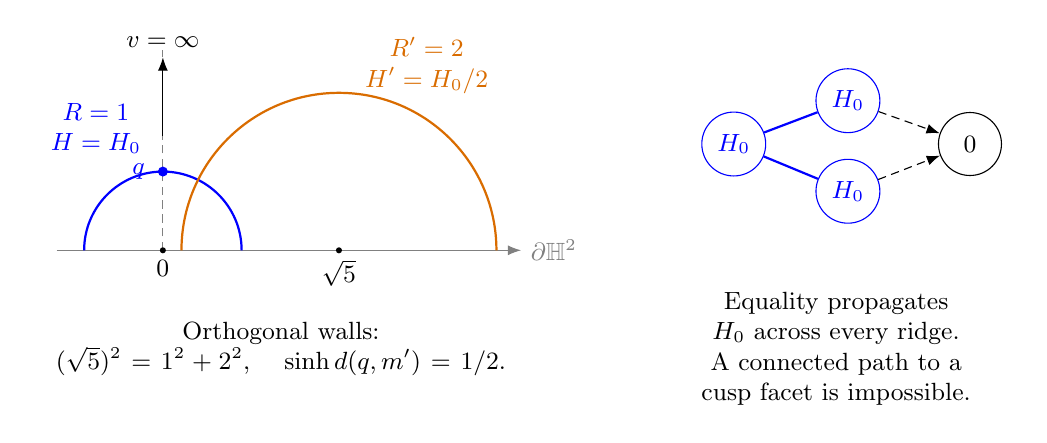
\begin{tikzpicture}[x=1.0cm,y=1.0cm,>=Latex,font=\small]
 \begin{scope}
  \draw[->,gray] (-1.35,0)--(4.55,0) node[right] {$\partial\HH^2$};
  \draw[thick,blue] (1,0) arc[start angle=0,end angle=180,radius=1];
  \draw[thick,orange!85!black]
   ({sqrt(5)+2},0) arc[start angle=0,end angle=180,radius=2];
  \draw[densely dashed,gray] (0,0)--(0,2.55);
  \draw[->] (0,1.45)--(0,2.45) node[above] {$v=\infty$};
  \fill[blue] (0,1) circle(1.8pt) node[left=3pt] {$q$};
  \fill (0,0) circle(1.1pt) node[below] {$0$};
  \fill ({sqrt(5)},0) circle(1.1pt) node[below] {$\sqrt5$};
  \node[blue,align=center] at(-.85,1.55) {$R=1$\\$H=H_0$};
  \node[orange!85!black,align=center] at(3.35,2.35)
   {$R'=2$\\$H'=H_0/2$};
  \node[align=center,text width=6.2cm] at(1.5,-1.25)
   {Orthogonal walls:\\
    $(\sqrt5)^2=1^2+2^2$, \quad $\sinh d(q,m')=1/2$.};
 \end{scope}
 \begin{scope}[xshift=7.25cm]
  \node[draw,circle,blue,minimum size=8mm] (a) at(0,1.35) {$H_0$};
  \node[draw,circle,blue,minimum size=8mm] (b) at(1.45,1.9) {$H_0$};
  \node[draw,circle,blue,minimum size=8mm] (c) at(1.45,.75) {$H_0$};
  \node[draw,circle,minimum size=8mm] (d) at(3,1.35) {$0$};
  \draw[blue,thick] (a)--(b) (a)--(c);
  \draw[densely dashed,->] (b)--(d);
  \draw[densely dashed,->] (c)--(d);
  \node[align=center,text width=4.4cm] at(1.3,-1.25)
   {Equality propagates $H_0$ across every ridge.\\
    A connected path to a cusp facet is impossible.};
 \end{scope}
\end{tikzpicture}
\caption{The left panel is a genuine upper half-plane section of two
orthogonal hemispherical walls, with the indicated radii. The right
panel records propagation on the facet graph; it makes no metric
assertion about a planar drawing of that graph.}
\label{fig:height}
\end{figure}

\section{A spherical code in the selected facet}

Every facet of $Q$ comes from exactly one actual ridge neighbor
$m_i$ of $n$. Because the dihedral angle is right, $m_i\in n^\perp$
and remains a unit vector for the intrinsic Lorentz form. Use $q$
as the time axis in this space. There are unit spatial vectors $u_i$
such that
\begin{equation}\label{eq:split}
 m_i=\bigl(t_i,\sqrt{1+t_i^2}\,u_i\bigr),
 \qquad u_i\in S^{n-2}.
\end{equation}

\begin{lemma}[The code bound]\label{lem:code}
Distinct neighboring walls give distinct $u_i$, and
\begin{equation}\label{eq:code}
 u_i\cdot u_j\le
 \frac{t_it_j}{\sqrt{(1+t_i^2)(1+t_j^2)}}\le\frac12.
\end{equation}
In dimension five, $Q$ has at most $24$ facets.
\end{lemma}
\begin{proof}
Apply~\eqref{eq:acute} to the two actual normals $m_i,m_j$ and
substitute~\eqref{eq:split}. Since $t_i,t_j\in[0,1]$, each factor
$t_i/\sqrt{1+t_i^2}$ is at most $1/\sqrt2$, proving the second
inequality. If $u_i=u_j$, then
\[
 \ip{m_i}{m_j}
 =-t_it_j+\sqrt{(1+t_i^2)(1+t_j^2)}>0,
\]
contrary to~\eqref{eq:acute}. Thus this is a code with as many
members as facets of $Q$. For $n=5$ it lies in $S^3\subset\RR^4$;
Proposition~\ref{prop:musin} gives the asserted bound.
\end{proof}

Suppose now that $P$ is entirely ideal and $n=5$. The four-facet $Q$
inherits entire ideality, finite volume and right angles. These
inheritance statements are used for a face of dimension four, not
for ideal polygon angles. Proposition~\ref{prop:kolpakov} and
Lemma~\ref{lem:code} give
\begin{equation}\label{eq:equality}
 24\le \#\{\text{facets of }Q\}\le24.
\end{equation}
Consequently $Q$ is a regular ideal right-angled $24$-cell.

\section{The equality point and global propagation}

We need a little more than the facet count. All neighbors must have
the same height, which follows from the metric equality case of
Proposition~\ref{prop:kolpakov}.

\begin{lemma}[The center is forced]\label{lem:center}
In a regular ideal right-angled $24$-cell, a future unit timelike point
whose products with all outward unit normals have negatives at most
one is the center. All those negatives then equal one.
\end{lemma}
\begin{proof}
In signature $(-,+,+,+,+)$ use the standard outward unit normals
\begin{equation}\label{eq:cellnormals}
 (1,\epsilon e_i+\delta e_j),\qquad
 1\le i<j\le4,\quad\epsilon,\delta\in\{1,-1\}.
\end{equation}
The center is $(1,0)$, and each normal has an opposite spatial
partner: $(1,r)$ and $(1,-r)$. Write the given point as $(a,w)$.
Then $a>0$, $a^2-\norm w^2=1$, and the two negatives are
$a-r\cdot w$ and $a+r\cdot w$. Their upper bounds by one imply
$2a\le2$. Future unit timelikeness implies $a\ge1$. Thus $a=1$
and $w=0$, as required.
\end{proof}

\begin{proof}[Proof of Theorem~\ref{thm:main}]
Assume first that $P$ is an entirely ideal right-angled five-polytope.
Fix the cusp representative $v$, height function and maximum $H_0$
as above. At any maximum-height facet the selected point $q$ lies
in the regular $24$-cell $Q$, by~\eqref{eq:equality}. All neighboring
heights satisfy $t_i\le1$. Lemma~\ref{lem:center} forces $q$ to be
the center, so every $t_i=1$. Formula~\eqref{eq:ti} therefore gives
\[
 H(m_i)=H_0
 \quad\text{for every facet adjacent to a maximum-height facet.}
\]

The set of maximum-height facets is nonempty and closed under facet
adjacency. The facet-adjacency graph is connected, so every facet
would have height $H_0>0$. This contradicts the height-zero facets
through the chosen cusp.

For completeness, connectivity here is the usual connectivity of
the facet graph of the compact projective convex closure of $P$.
This is a finite Euclidean polytope with the same face lattice.
Its positive-dimensional ridges have hyperbolic relative interior,
so the graph edges are precisely the actual ridge adjacencies used
in the proof; cusp-only contacts do not serve as graph edges.

There is therefore no entirely ideal right-angled five-polytope.
In every higher dimension a five-face would inherit finite volume,
entire ideality and right angles, giving the same contradiction.
The regular ideal right-angled $24$-cell supplies the example in
dimension four.
\end{proof}

The argument uses no field restriction, local search, numerical
optimization or assumed classification of higher-dimensional
polytopes. Its two numerical inputs are exactly
Propositions~\ref{prop:musin} and~\ref{prop:kolpakov}. The all-wall
check~\eqref{eq:allwalls}, the allowed zero heights, and the explicit
opposite-normal calculation are included to keep projection and
equality independent of any informal picture.

\begin{thebibliography}{9}
\bibitem{Kolpakov}
A. Kolpakov, \emph{On the optimality of the ideal right-angled
$24$-cell}, Algebraic \& Geometric Topology \textbf{12} (2012),
1941--1960.
\href{https://doi.org/10.2140/agt.2012.12.1941}{doi:10.2140/agt.2012.12.1941}.

\bibitem{Musin}
O. R. Musin, \emph{The kissing number in four dimensions}, Annals of
Mathematics (2) \textbf{168} (2008), 1--32.
\href{https://doi.org/10.4007/annals.2008.168.1}{doi:10.4007/annals.2008.168.1}.

\bibitem{Vinberg}
E. B. Vinberg, \emph{Hyperbolic reflection groups}, Russian Mathematical
Surveys \textbf{40}:1 (1985), 31--75.
\href{https://doi.org/10.1070/RM1985v040n01ABEH003527}{doi:10.1070/RM1985v040n01ABEH003527}.
\end{thebibliography}
\end{document}
